\section{Introduction}
\label{introduction}

Implantable medical devices like pacemakers are designed to improve certain undesired physiological conditions with very little human interventions. 
Their ability of autonomously affect the physiological conditions of the patients makes the medical devices safety-critical, and sufficient evidence on the safety and efficacy of the devices should be provided before the devices can be implanted in the patients. 
As more functions added to the devices, the complexity of the software component of the device is increasing dramatically, leading to increasing number of potential safety violations due to software bugs. 
\todo{give recall statistics}
In what follows, we use the word `device' to refer both to the hardware and the software of the device.

There are two categories of device bugs: 
first, the device may fail to conform to its \emph{specification}, i.e. the prescription of how it should react to certain inputs.  
Secondly, even if it conforms to its specification, the device may fail to improve the health of the patient as promised. 
The improved state of health is captured in the \emph{physiological requirements}; e.g., for a pacemaker, the heart rate should always be below a certain threshold. 
%In what follows, the word `requirement' always refers to such physiological requirements.
Note that requirements are about \emph{the closed-loop system}: they prescribe the behavior of both device and environment (e.g. both pacemaker and heart).

Bugs in the first category (non-conformance to specification) are detected via extensive open-loop testing where a set of input sequences is fed to the device, and its output is observed to see if it matches the expected output.
Bugs in the second category (violation of physiological requirements), on the other hand, require the availability of the closed-loop system: e.g., the heart and the pacemaker. 
In the medical device industry, clinical trials amount to a closed-loop test of the device and its software. 
In a clinical trial, the actual device is implanted in a human subject and its operation tested over a certain duration.
Unfortunately, clinical trials can only cover a very limited range of physiological conditions due to their extremely high cost. 
\todo{give dollar amount}
Moreover, clinical trials are often conducted at the last design stage. Fixing bugs at this stage is also very costly.

On the other hand, using a virtual model of the device's environment, we can conduct \emph{model-based clinical trials}: i.e., the device (or a model thereof) is connected to a virtual model of the environment and this virtual closed loop is verified.
Depending on the formalism used to model the environment (and device) and the language used to express the requirements, this allows the usage of formal methods to perform the verification.
Environment modeling introduces new challenges and issues that do not arise when modeling the device alone, and this paper aims at addressing these issues in the context of pacemaker verification.
The proposed method is also generalizable to other contexts where closed-loop formal verification is desired.
In the rest of this paper, we speak therefore of pacemaker as the Device Under Verification (DUV) and of the heart as being the environment, but it is understood that the discussion carries more broadly, with possible domain-specific adjustments.

The first challenge in closed-loop verification of pacemakers is that the human heart displays a large number of different conditions, henceforth referred to as `physiological conditions'.
E.g., one heart may display \emph{atrial fibrillation} where the upper chambers of the heart (the atria) produce an exceedingly fast beat that prevents proper blood pumping.
Another heart may display Premature Ventricular Contraction (PVC) where a location in the ventricles produces electrical impulses at erratic time instants.
Each such condition will require its own formal model, and some models may display more than one condition.
In this paper, we build such a set of formal heart models using a network of timed automata in Section ???.
Model checking for timed automata is decidable [???].
Rather than perform verification on each model separately, we seek a method that can combine models, and perform model checking on the merged model. 
The combination of models must be such that if the merged model is correct (according to the requirements) then so is every model that was combined into it.
We present \emph{abstraction rules} in Section ?? which allow us to do precisely that.

This initial set of models will necessarily be incomplete because the number of conditions is too large, and some of the conditions are too ill-understood for modeling.
Thus, unlike system modeling where one typically starts from one ground truth model to be verified, our starting point is an \emph{incomplete set of models}.
In typical formal verification practice, when the state space of a model $M$ is too large, \emph{predicate abstraction} is used to reduce the size of the state space while still preserving all the behavior of the original model. 
This reduction in size may allow model checking where it wasn't possible before. 
Because the abstract model $M'$ also introduces new behavior that didn't exist in the ground truth $M$, this new behavior is rejected as \emph{spurious} if it is encountered, and the abstraction is refined.
This is the familiar CEGAR procedure[???].
However when modeling the environment, we use abstraction differently. 
Because we start from an \emph{incomplete} set of models, we would like our abstraction procedures to introduce new \emph{physiologically meaningful} behavior which might actually be produced by heart models not in the initial set.
These then correspond to heart conditions not taken explicitly into account. 
This motivates the introduction of domain-specific abstraction rules $R$ in Section ???: like predicate abstraction, they produce models that over-approximate the behavior of the model they are applied to (i.e., $\beh(R(M)) \supset \beh(M)$).
However, the new behavior they introduce might not be spurious. 
We demonstrate such a case in Section ???.
If model checking returns a counter-example on $R(M)$, the physician can decide whether this is actually physiologically plausible behavior and therefore the pacemaker needs to be debugged, or this is indeed spurious and should be thrown out (and the abstraction refined).

%Moreover, because our models are timed automata, the model checking procedure already applies predicate abstraction to the clocks to obtain a symbolic checkable model [???], so that further abstraction is not possible.\todo{delicate...make sure it doesnt' go against the argument so far}
Moreover, because we start from a set of initial models, and use a set of abstraction rules, we actually produce an \emph{abstraction tree} rather than an abstraction chain.
We demonstrate the construction and use of such a tree for the formal verification of pacemakers in Section ???

\subsection{Technical preliminaries}
In this section we briefly review the notions of abstraction and over-approximation of system.
Let $M$ be a system model and $S$ be its state space (in Section ??? we give a specific formalism in which our systems are modeled).
A \emph{trace} $\straj$ of $M$ is an infinite sequence of states produced by $M$: $\straj \in S^\omega$.
The \emph{behavior} $\beh(M) \subset S^\omega$ of $M$ is then the set of all its possible traces.

Let $AP$ be a set of atomic propositions and $\phi$ be an ACTL$^*$ formula over $AP$ [???].
ACTL$^*$ is the fragment of CTL$^*$ with only the universal quantifier (``for every path'').
The set of $M$ traces that satisfy $\phi$ is denoted by $\beh(\phi)$. 
It holds by definition that if $M$ satisfies $\phi$, then $\beh(M) \subset \beh(\phi)$.
We write this as $M \models \phi$.
A model checker takes $M$ and $\phi$ as inputs and either returns SAT, meaning that $M \models \phi$, or returns a \emph{counter-example}, which is a trace $\straj \in \beh(M) \setminus \beh(\phi)$.

An \emph{abstraction function} $\absfun: S \rightarrow S'$ maps the states of $M$ to new \emph{abstract} states.
We extend it to traces and sets of traces in a natural manner: $\absfun(\straj) =  \absfun(s_0)\absfun(s_1)\ldots$ for $\straj = s_0 s_1\ldots \in S^\omega$,
and $\absfun(W) = \cup_{\straj \in W}\absfun(\straj)$ for any $W \subset S^\omega$.
The abstraction function is total (i.e. defined for every $s \in S$) and is such that
\[R(\beh(M)) \subset \beh(M') \]
where $\absfun(W) = \cup_{\straj \in W} \absfun(\straj)$.
Abstraction is used to reduce the size of the state space ($|S'| < |S|$), so that model checking becomes feasible on the new model $M'$ with state space $S'$, while preserving behavior.
Indeed, if $R(\beh(M)) \subset  \beh(M') $ and $\beh(M') \subset \beh(\phi)$, then it holds that $\beh(M) \subset \beh(\phi)$ and so $M \models \phi$ (here we omit certain technicalities relating to the appropriateness of the abstraction function $\absfun$ to $\phi$. The reader is referred to [Section 3, Clarke JACM] for a good overview).

A \emph{closed loop requirement} is an ACTL$^*$ formula $\formula_C$ of the form $\formula_C :=\formula_E \implies \formula_D$ in which $\formula_E$ describes the open-loop environment behavior that the device encounters, and $\formula_D$ is the closed-loop behavior that the device should achieve. 

A \emph{closed loop requirement} is an ACTL$^*$ formula of the form$\formula_E\Rightarrow \formula_C$ where $\formula_E$ is a specification on the environment model and $\formula_C$ is a specification on the closed-loop model.
For example, 
\[\textrm{AtrialSense} \implies \eventually ((\textrm{VentricularSense } ||  \textrm{ VentricularPace }) \land  t \leq 500)\]
 expresses that if the heart displays electrical activity in the atrium (an `atrial sense'), then there should be electrical activity in the ventricles within 500ms (either naturally or as a result of a pacing event).

\subsubsection{Spurious vs physiologically valid counter-examples}
Suppose a model checker is run on an abstract model $M'$ obtained by abstracting $M$ using some abstraction function $R$.
If the checking returns a counter example $\straj \in \beh(M')$, two cases are possible:
either $R^{-1}(x) \in \beh(M)$, or not.
In the first case, there is no ambiguity: this is a valid counter-example.
In the second case $R^{-1}(x) \notin \beh(M)$, the trace $\straj$ is usually discarded as being spurious.
This makes sense if the model $M$ is taken to be the ground truth: i.e. anything not generated by $M$ is not valid behavior. 
However, when modeling the environment as we need to for closed-loop verification, $M$ is only one of many models, none of which is ground truth. 
That is, it is recognized that there exists physiologically meaningful behavior not captured by any of the models. 
In this case, we use abstraction functions not only to reduce the size of the state space, but mainly to \emph{introduce, in a systematic manner, physiologically meaningful behavior}. 
Thus a counter-example $\straj$, while not producable by any of the initial models, may still be a valid example.
\begin{figure}[!t]
		\centering
		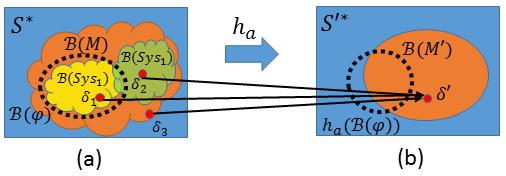
\includegraphics[width=0.8\textwidth]{figs/distinction.png}
		%\vspace{-5pt}
		\caption{\small Two models such that $\{Sys1,Sys2\}\triangleleft_h M$. An abstraction function $h_a$ is applied to $M$ to obtain $M'$. By model checking the abstract model $M'$ against property $\formula$ we have $M'\not\models\formula$ and $\delta'$ is returned as counter-example. However, $\delta'$ corresponds to 3 different behaviors in the original behavior space: $\delta_1$ satisfied and valid; $\delta_2$ unsatisfied and valid; $\delta_3$ unsatisfied and invalid}
		  %\vspace{-15pt}
		\label{fig:ambiguity}
\end{figure}

\subsection{System Modeling vs. Environment Modeling}
During closed-loop model checking, there are different focuses on the system model and the model of its environment, thus modeling them require different strategy.
\subsubsection{Over-approximation: }In closed-loop model checking, there is only one concrete system. However there can be countless number of environmental conditions which require different models to represent. While over-approximating the system model aim to reduce its state space and computational cost, over-approximating the environment models aim to cover the behaviors of multiple environmental conditions that are explicitly modeled, or implicitly included. Since it is impossible to exhaustively model all possible environment conditions, over-approximation is a good way to cover multiple environment condition without increasing computational cost. %\figref{distinction}

\subsubsection{Validity of a counter-example: }Behaviors introduced into the over-approximation of a system model are all \emph{spurious}, or invalid. For two models such that $M\triangleleft_h M'$, $\delta'$ is spurious if the following condition holds: 
$$\not\exists \delta\in\mathbb{B}(M) \text{ s.t. }h(\delta)=\delta'$$
However, for environment models such that $\{M_1,M_2,...M_n\}\triangleleft_h M'$, and an execution $\delta'\in\mathbb{B}(M')$, the following condition is not enough to prove $\delta'$ is spurious.
$$\forall i\not\exists \delta\in\mathbb{B}(M_i)\text{ s.t. }h(\delta)=\delta'$$
Since there may be a valid environment model $M_c\not\in\{M_1,M_2,...M_n\}$ and $\mathbb{B}(M_c)\subset\mathbb{B}(M')$ and $\delta'\in\mathbb{B}(M_c)$. It is thus up to the domain experts to determine the validity of the counter-example.
%\begin{figure}[!b]
%		\centering
%		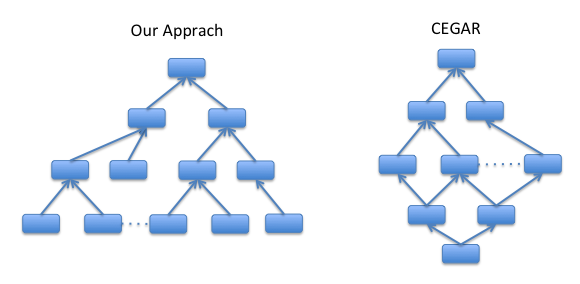
\includegraphics[width=0.6\textwidth]{figs/env_sys.png}
%		%\vspace{-5pt}
%		\caption{\small }
%		  %\vspace{-15pt}
%		\label{fig:distinction}
%\end{figure}

\subsection{Counter-Example-Guided Abstraction and Refinement (CEGAR)}
In \cite{CEGAR} the authors proposed a framework to over-approximate the system using proposition abstraction. Upon property violation the abstract counter-example is checked for its validity on the system. If the counter-example is spurious the model is then refined to eliminate the spurious counter-example. This process is then resumed on the refined model until either a valid counter-example returns or no counter-examples are returned.

From the above procedure we can see that CEGAR framework works on system modeling. However, CEGAR cannot be applied for environment modeling for the following reasons. First, the proposition abstraction can not over-approximate multiple models into one abstract model. 
%Proposition abstraction only abstract the domain of the substates and the dimensions of the state space is unchanged. For environment models with different substates, more aggressive abstraction functions are needed to over-approximate
With multiple environment models the validity of counter-examples cannot be determined by concretizing them on the set of environment models, as discussed in the last section. If over-approximation is used for environment modeling, there needs to be a more suitable framework to balance the abstraction and refinement of the environment models.

\subsection{Abstraction-tree-based Model Abstraction for Environment Modeling}
In this paper we propose framework for environment modeling in closed-loop model checking of medical device software. An incomplete set of physiological models are first developed to represent different physiological conditions. 

A set of physiological abstraction rules are then developed based on physiological knowledge, which ensure the physiological relevance of the behaviors introduced into the abstract models. 

Then the rules are applied in certain order onto the set of physiological models, resulting an abstraction tree $G=(V,E)$. Each leaf in the tree is a physiological model and the edges are applications of an abstraction rule. The abstraction tree can then be used as environment models for closed-loop model checking.

The closed-loop requirement $\formula_c:(\formula_E\Rightarrow\formula_P)$ has constraints on the environment in $\formula_E$. During the abstraction steps, certain sub-states or transitions of the environment models may be removed or merged. If the variables mentioned in $\formula_E$, which is denoted as $Var(\formula_E)$, is not a subset of the variables of an environment model $M$, which is denoted as $Var(M)$, the model $M$ is not appropriate for the requirement $\formula_c$. The first step for closed-loop model checking is to choose the most abstract environment model(s) from the tree which are appropriate for the requirement. These models will be used as the initial environment models $M_E$ during model checking. 

For a system model $M_S$ and a physiological requirement $\formula_c$, closed-loop model checking is performed such that:
$$\forall M\in M_E, \text{ check } M||M_S\models\formula_c$$
If the requirement is all satisfied, the system model $M_S$ satisfy $\formula_c$ under environment condition covered by the models in $M_E$. Upon violation of the requirement, the model checker returns a counter-example $\delta_c\in M_c\in M_E$. However, counter-examples at the abstract level are difficult to interpret and there may exists ambiguities. To concretize the counter-example and enumerate possible physiological context, we explore the abstraction tree. Model checking is then performed such that:
$$\forall M\in Child(M_c), \text{ check } M||M_S\models\formula_c$$  
The procedure recurs until 1) the leaves of the tree is reached, or 2) there is no violations in the child nodes. The counter-examples returned from the most refined models are then submitted to the physicians for analysis. 

%\todo[inline]{why give new names to familiar things? Especially since these names don't make sense at this point. E.g. you speak of validity ambiguity, but it is not at all clear what is being validated and why the equation expresses an `ambiguity'. This is basically a description of what happens when abstracting, which most formal people are familiar with, so merge with section \ref{MCproblem}}



%During the software development process, there are two key documents that track the safety and efficacy of the software component, namely the \textbf{Software Requirements} and \textbf{Software Specifications}. These two terms are sometimes used interchangeably, however, requirements and specifications provides different angle of system safety and require very different verification techniques.
%
%A requirement states the objective of the system in design in terms of environmental conditions. For example, a requirement of a self-driving car would be: \emph{The car should not hit a pedestrian.} A specification is how the system developers propose to satisfy the requirements. For example, the specification corresponding to the requirement of a self-driving car would be: \emph{If an object is detected in front of the car and the distance to the object is less than $d$, the car should brake.} As we can see, a specification may not satisfy the corresponding requirement, thus two steps are required to guarantee the safety of the system software. The first is the conformance between the system software and the software specification. The second one is whether the software specifications can satisfy all the software requirements.
%
%Currently in most system design, the conformance between the software specifications and the system software are verified using extensive \textbf{open-loop} testing. The test cases are extracted from the system software using static analysis based on certain coverage criteria. The conformance between the specifications and the requirements are maintained by traceability documents, which is insufficient for safety guarantee.
% \begin{figure}[!t]
% 		\centering
% 		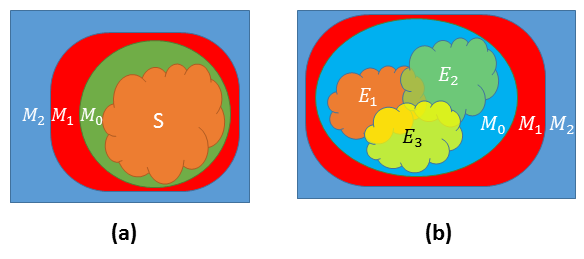
\includegraphics[width=0.8\textwidth]{figs/SysVSEnv.png}
% 		%\vspace{-5pt}
% 		\caption{\small Modeling in terms of behavior coverage. As model becomes more abstract, the coverage increases while the boundary becomes more simple. (a) System modeling in which there is only one concrete system; (b) Environment modeling in which abstraction can be used to generalize different conditions}
% 		  %\vspace{-15pt}
% 		\label{fig:sys}
% \end{figure}





\subsection{Contributions}
\label{contributions}
\begin{itemize}
	\item Highlighting the differences between verifying requirement vs. verifying specification and identified potential complications
    \item Emphasize model abstraction and refinement on environment model
    
    \item Define abstraction rules in terms of its effects on state transitions instead of states
    \item Document the following information during abstraction rule applications:
    
\begin{itemize}
	\item New grouping of state transitions
    \item Assumptions made that may increase environment behaviors
\end{itemize}
    \item Use state transitions to describe environmental behaviors and even requirements
    \item Identify the possibility and necessity to refine the model from requirement point of view
    \item For any closed-loop requirement, (semi-) autimatically identify the most abstract environment model that can unambigurously describe the environmental constraints in the requirement.
    \item Apply the requirement-guided approach on a pacemaker case study
    \item Developed a Matlab toolbox for suggesting EP heart models during closed-loop model checking of pacemaker software
\end{itemize}


%\paragraph{Notation}. For a positive integer $n$, $[n] = \{1,2,\ldots,n\}$.

%\section{Closed-loop Model Checking}
%We first define the behavior space of a model as all combinations of states valuations. For a model $M$ with $n$ state variables $v_1\dots v_n$, and each state variable can take value within the domain $D(v_i)$, the size of the overall behavior space is $\Pi_{i=1}^n D(v_i)$. The actual reachable behavior space of a model $M$ is far less and can be defined by $\mathbb{B}(M)$. As a reference or ground truth for behavior space, we assume the behavior space $\mathbb{B}(S)$ for a physical system $S$ which is infinitely large. All the behavior spaces correspond to the models $\mathbb{B}(M)$ of the system are projections from $\mathbb{B}(S)$.  
%\Hao{}
For a model $M$ with state space $S$, we define the behavior of the system as an execution trace in $\delta\in S^*$. The reachable behavior space of model $M$ is denoted as $\mathbb{B}(M)\subset S^*$. For reference we can represent an actual system as a model $M_t$ with infinite details. A property defines a region in the behavior space within which the property is satisfied. The satisfaction region of a property $\varphi$ can be denoted as $\mathbb{B}(\varphi)$. A system $M_t$ satisfies a property $\varphi$ if $\mathbb{B}(M_t)\subseteq \mathbb{B}(\varphi)$. We denote it as $M_t\models\varphi$. 

Models can be abstracted to potentially reduce complexity and increase coverage. An abstraction function $h$ abstracting model $M$ to $M'$ is a non-surjective function from state space $S$ to the new abstract state space $S'$ such that 
$$\forall s\in S, \exists s'\in S' \text{ s.t. } h(s)=s'$$
For a behavior $\delta\in \mathbb{B}(M)$
$$\forall \delta\in \mathbb{B}(M),\exists \delta\in\mathbb{B}(M')\text{ s.t. } h(\delta)=h(\delta')$$
The abstract model $M'$ covers all behaviors of $M$, which is referred to as \emph{over-approximation}. 
As we can see, if $M$ is an over-approximation of $M_t$, meaning $\mathbb{B}(M_t)\subseteq \mathbb{B}(M)$, and $\mathbb{B}(M)\subseteq \mathbb{B}(\varphi)$, we have:
 $$\mathbb{B}(M_t)\subseteq \mathbb{B}(\varphi)\rightarrow M_t\models\varphi$$ 
Since the state space of $S'$ is smaller than $S$ while still preserve the property, during model checking the more abstract model can be used to check the property. 

Since $h$ is non-surjective, 

%No models of the system can match the region of the system exactly due to lack of information. As the model becomes more abstract, the boundary defining the behavior region becomes less complex. If the abstract model covers all the system behaviors such that $\mathbb{B}(S)\subset\mathbb{B}(M)$, the model is referred to as an \emph{over-approximation} of the system. For environment model, over-approximation can also be used to \emph{generalize} different environmental conditions, i.e. in \figref{distinction}.(a) two system behaviors $\mathbb{B}(S_1)$ and $\mathbb{B}(S_2)$ are covered by a model $\mathbb{B}(M)$.


In most of the cases, the internal states and transitions of a system cannot be fully observable. The behavior space can thus be mapped to other observable behavior spaces with less dimensions.
\Hao{Need to clarify/visualize the notion of observability here} 
Note that the observability does not refer to the interface of the system, there can be multiple observable behavior spaces that correspond to different abstraction of the system. As the result, behaviors that are distinguishable in the full behavior space can be indistinguishable in a observable behavior space, causing ambiguities that can result in false-negatives and false-positives during verification. We denote one observable behavior space as $\mathbb{B}_o(S)$. 

As shown in \figref{distinction}, $\mathbb{B}(M)$ and $\mathbb{B}(\varphi)$ are mapped to $\mathbb{B}_o(M')$ and $\mathbb{B}_o(\varphi')$. Three behaviors in $b_1,b_2,b_3\in\mathbb{B}$ are mapped to a single behavior $b'\in\mathbb{B}_o$. Since $b'\not\in\mathbb{B}_o(\varphi')$, it may be returned by verification tools like model checker as counter-example. In $\mathbb{B}_o$ is possible that two categories of ambiguities exist, namely \textbf{Validity ambiguity} and \textbf{Context ambiguity}. %Failure to distinguish these behaviors can cause false-negatives and/or false-positives during verification.

Validity ambiguity refers to the incapability to distinguish a physically possible execution with an invalid one. In \figref{distinction}.(a), $b_3$ is an invalid behavior since it does not belong to either $S_1$ or $S_2$ but it is covered by the model $M$. 

A model $M$ is compatible with an observable behavior space $\mathbb{S}^o$ if all the behaviors that can be generated by $M$ 

A model is appropriate for a property if all its behaviors  



A Counter-Example-Guided Abstraction and Refinement approach has been proposed to automatically derive model with appropriate amount of details. (\cite{CEGAR}) Assume we would like to check the system $S$ against the property $\varphi$. First, the most abstract model $M_0\models^a S$ is derived from the actual system $S$ based on certain abstraction rules, so that it can distinguish all execution paths that satisfy/violate $\varphi$. Then $M_0$ is verified against the property in an automated model checker. If the property is violated $M_0\not\models\varphi$, a counter-example $\delta^c$ is returned by the model checker. $\delta^c$ has to be then validated so that it can be produced by $S$. If the system can produce $\delta^c$, which can be denoted as $\delta^c\triangleleft S$, $\delta^c$ is a valid counter-example. Otherwise $\delta^c$ is regarded as \textbf{spurious} and the model has to be refined so that the $\delta^c$ is not producible by the model. The refined model $M_1\models^a M_0$ is derived by adding back the minimum amount of abstracted details that prevent $\delta^c$ from being enabled, so that $\delta^c\not\triangleleft M_1$. This process continues until either no counter-example is returned, or a counter-example is not spurious. 

CEGAR works very well during system modeling in which there is only one concrete system implementation $S$. However, for closed-loop verification the objective is to check whether $E||S\models\varphi$. If the environment $E$ is also represented by a model during model checking, both $M^E$ and $M^S$ have to be unambiguous. When verifying system specifications, normally there is no constraints on the environment so that there is no spurious counter-examples due to the environment model. In this case CEGAR still works. However in the software requirements, there are constraints on the environment conditions. If these constraints are not enforced in $M^E$, the verification can yield spurious counter-examples. However, CEGAR will not work for environment modeling due to the differences between the environment and the system. In system modeling, there is only one concrete implementation $S$, so if a counter-example $\delta^c$ is returned during model checking, only $\delta^c\triangleleft S$ has to be checked. However, for the environment, there are infinite number of environmental conditions $E_i$, like different patients in the medical device domain. Details are ignored in the abstract models not only to reduce complexity, but also to \textbf{generalize} different conditions so that:
$$\forall \delta\triangleleft E_i, i\in [1,n],\delta\triangleleft M^E$$
Note that during the generalization process, more behaviors of the environment will be introduced into the model: 
$$\exists\delta^s\triangleleft M^E \text{ s.t. } \delta^s\not\triangleleft E_i, i\in [1,n]$$
In this case, if an execution path $\delta$ is returned as a counter-example during model checking on software requirement, there is no way to check whether 
$$\exists i\in[1,n],\delta\triangleleft E_i$$ 
as $n$ may be a large number or is unclear in the first place. As a result, the validity of the counter-example cannot be validated, and therefore the model cannot be refined by analyzing the spurious counter-example. CEGAR is not effective during environment modeling.

In Cyber-Physical Systems, there are \textbf{domain experts} who understand how the environment of the system works. The \textbf{domain knowledge} is a set of environmental constraints which can be used to define different environment conditions, and determine the validity of the execution paths. However, domain knowledge are in general not formalized thus cannot be used in any automated processes. In this paper, we use closed-loop model checking on an implantable pacemaker model as example to demonstrate abstraction and refinement of the environment models using encoding domain knowledge. We use two case studies to demonstrate that although CEGAR is not applicable to the environment model, the domain knowledge can still be used to validate executions and provide potential validity violations.\Hao{Still need to formalize}

The contribution of this paper is two-folds: 1) we formally specified the potential ambiguities during model abstraction and identified the difference between environment modeling and system modeling. 2) We demonstrated the potential application of encoded domain knowledge to eliminate the ambiguities during abstraction and refinement of environment models.
\begin{itemize}
	\item Abstraction rules for environment models 
    \item Appropriate abstraction function check, definition clear, assumptions implicit, especially for environment models
\end{itemize}
%\section{A Simple Example}
Imaging we are developing a high-level control algorithm for an autonomous vehicle
\textsf{A[] (not CarCross $\&\&$ PedCross)}\\
\textsf{E<> (CarCross)}
\begin{figure}[!t]
		\centering
		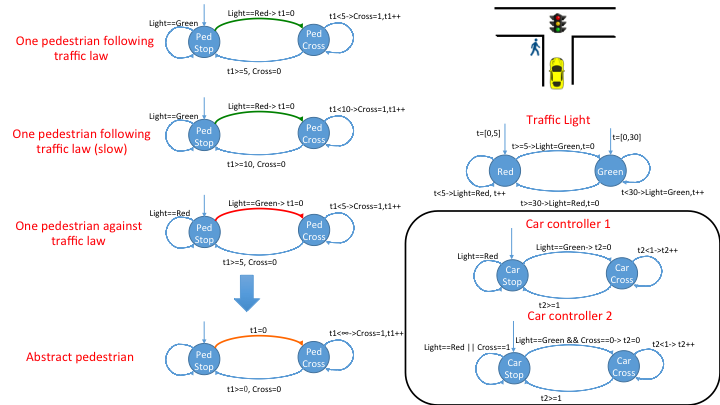
\includegraphics[width=0.9\textwidth]{figs/example.png}
		%\vspace{-5pt}
		\caption{\small }
		  %\vspace{-15pt}
		\label{fig:example}
\end{figure}